\chapter{Introduzione}

\section{Problemi computazionali}

\dfn{Problema computazionale}{
  Un \textbf{\textit{problema computazionale}} è una \textit{collezione di domande} per cui sia stabilio un criterio per riconoscere le risposte corrette.
}

\ex{Problema computazionale come collezione di domande}{
  \subsubsection{Massimo Comune Divisore}
\begin{itemize}
  \item Ingressi:
  \begin{itemize}
    \item [$\Rightarrow$] Coppie di interi positivi $a$, $b$ non entrambi nulli.
  \end{itemize}
\item Uscite:
    \begin{itemize}
    \item [$\Rightarrow$] Un intero positivo $c$ tale che $c$ divide sia $a$ che $b$ e se un intero positivo $d$ divide $a$ e $b$ allora $d \leq c$. 
  \end{itemize}
\end{itemize}

}

\nt{Però la definizione sopra è "intuitiva", per cui si necessità di una formalizzazione.}

\dfn{Problema computazionale}{
  Un \textbf{\textit{problema computazionale}} è una \textit{relazione binaria}, cioè un insieme di coppie ordinate in cui ogni coppia è composta da un ingresso (la domanda) e l'uscita corrispondente (la risposta).
}

\cor{Dominio}{
  Il \textbf{\textit{dominio}} è l'insieme di istanze che hanno una risposta. 

  $dom\{R\} = \{i|\exists r. (i, r) \in R\}$
}

\cor{Univocità}{
 Un problema computazionale è \textbf{\textit{univoco}} se ogni istanza ammette una e una sola soluzione.
}

\begin{figure}[h]
    \centering
    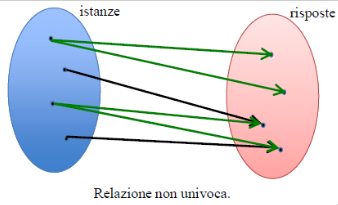
\includegraphics[scale=0.5]{1/RelNu.png}
    \caption{Esempio di relazione non univoca.}
\end{figure}

\ex{Problema computaionale come relazione binaria}{
  \subsubsection{Massimo Comune Divisore}
  $$R = \{((a, b), c) | a \in \bbZ \land b \in \bbZ \land (a > 0 \lor b > 0) \land a \texttt{ mod } c == 0 \land b \texttt{ mod } c == 0 \land$$ $$ (\forall d > 0 (a \texttt{ mod } d == 0 \land b \texttt{ mod } d == 0) \Rightarrow d \leq c)\}$$
}

\subsection{Algoritmi}

\dfn{Algoritmo}{Un \textbf{\textit{algoritmo}} è un metodo meccanico per risolvere un problema computazionale.}

\cor{Procedura}{Una \textbf{\textit{procedura}} è una sequenza finita di operazioni meccanicamente eseguibili, per produrre univocamente un'uscita a partire da certi ingressi.}

\nt{Un algoritmo può essere visto come una procedura che termina per ogni ingresso ammissibile.}

\dfn{Determinismo}{
Un algoritmo è \textbf{\textit{deterministico}} se eseguito più volte sullo stesso input fornisce lo stesso output. A ogni algoritmo deterministico è associata una \textit{funzione} dagli ingressi alle uscite.
}

\cor{Correttezza}{
  Un algoritmo risolve un problema computazionale R, ossia è \textbf{\textit{corretto}} rispetto a R, se, la coppia formata dall'input (generico) e dal corrispondente output è in R.
}

\nt{Il primo algoritmo fu proprio quello che calcola il massimo comune divisore, comunemente noto come "Algoritmo di Euclide".}

\asd{Euclide}{

\begin{center}
    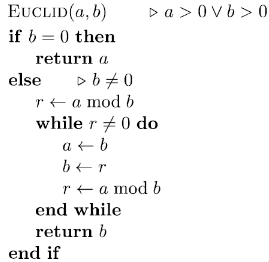
\includegraphics[scale=0.65]{1/Eu.png}
\end{center}
}

\dfn{Programma}{
  Un \textbf{\textit{programma}} può contenere diversi algoritmi. Un programma è scritto in uno specifico linguaggio di programmazione, per cui occorre specificare e implementare diverse \textbf{\textit{strutture dati}} $\Longrightarrow$ PROGRAMMA = ALGORITMI + STRUTTURE DATI.
}

\subsection{Problemi impossibili e molto difficili}

\qs{}{Tutti i problemi computazionali ammettono una soluzione algoritmica?}

\paragraph{Risposta:} No, esistono problemi \textit{indecidibili}. 

\dfn{Halting problem}{
  È possibile sviluppare un algoritmo che, dato un programma e un determinato input finito, stabilisca se il probblema termini o continui la sua esecuzione all'infinito?
}

\nt{La risposta è semplicemente \textbf{\textit{no}}.}

\dfn{Problema intrattabile}{
  Un \textbf{\textit{problema intrattabile}} è un problema per il quale non esiste un algoritmo con complessità polimoniale in grado di risolverlo.
}

\cor{NP-completezza}{
  Classi di problemi tali che tutti o nessuno ammettono una soluzione in tempo polinomiale.
}

\nt{I problemi intrattabili e la questione P=NP vengono affrontati in dettaglio nel corso "Calcolabilità e Complessità".}


\section{Correttezza e Terminazione}

\subsection{Correttezza e Logica di Hoare}

Bisogna verificare la \textbf{correttezza} degli algoritmi (e dei programmi che li implementano). 

\dfn{Correttezza totale}{
  Un algoritmo è \textbf{\textit{corretto}} se per ogni input fornisce l'output corretto. 
}

\nt{Tuttavia questa definizione spesso è troppo "forte".}

\dfn{Correttezza parziale}{
  Un algoritmo è \textbf{parzialmente corretto} se per ogni input \textit{se termina} fornisce l'output corretto.
}

\nt{La correttezza parziale viene molto approfondita nel corso "Metodi Formali dell'Informatica" in cui si va a costruire un verificatore per programmi che terminano (utilizzando la logica di Hoare).}

\dfn{Logica di Hoare}{
  La logica di Hoare si compone di:
  \begin{itemize}
    \item [$\Rightarrow$] Precondizioni: che devono essere vere prima dell'esecuzione dell'algoritmo;
    \item [$\Rightarrow$] Postcondizioni: che devono essere vere al termine dell'esecuzione dell'algoritmo.
  \end{itemize}

}

\ex{Logica di Hoare}{
  \subsubsection{Divisione intera}
\begin{itemize}
  \item Precondizioni:
  \begin{itemize}
    \item [$\Rightarrow$] $a \geq 0$, $b > 0$ numeri interi. 
  \end{itemize}
\item Postcondizioni:
    \begin{itemize}
    \item [$\Rightarrow$] Il risultato è un intero $q$ tale che $a = b * q + r$ con $0 \leq r < b$.
  \end{itemize}
\end{itemize}


}

\subsection{Induzione}

\dfn{Induzione semplice}{
  Una proprietà $P(n)$ che vale per $n = 0$ (passo base) e se vale per $n$ allora vale anche $n + 1$ (passo induttivo\footnote{Anche detto passo ricorsivo}) vale per ogni $n \geq 0$.


  $$(P(0) \land (\forall n \in \bbN. P(n) \Longrightarrow P(n + 1))) \Longrightarrow \forall n \in \bbN. P(n)$$
}

\cor{Generalizzazione dell'induzione semplice}{
  Il passo base può anche essere un generico $k$ diverso da 0. 

 $$(P(k) \land (\forall n \geq k. P(n) \Longrightarrow P(n + 1))) \Longrightarrow \forall n \geq k. P(n)$$

}

\nt{Inoltre il passo induttivo può anche avere forma $P(n - 1) = P(n)$.}

\ex{Dimostrazione con induzione semplice}{
  Dimostriamo che $\sum_{k = 1}^n = (2k -1) = n^2$

  \begin{itemize}
    \item [$\Rightarrow$] Passo base: si parte da 1 (il primo valore assegnato a $k$) e si termina sempre con 1 ($n = 1$)

      $$\sum_{k=1}^1 (2k - 1) = 1^2 = 1$$

    \item [$\Rightarrow$] Passo induttivo: supponiamo che la proprietà sia vera per $n$ 

    $$\sum_{k=1}^{n + 1} (2k - 1) = \sum_{k=1}^n (2k - 1)) + (2(n +1) - 1) = n^2 + 2n + 1 = (n + 1)^2$$
  \end{itemize}
}

\dfn{Induzione completa}{
  Una proprietà $P(n)$ che vale per $n = 0, 1, ..., k$ (passo base) e se vale per $0, 1, ..., n$ allora vale per $n + 1$ (passo induttivo) vale per ogni $n \geq 0$. 


  $$(P(0) \land P(1) \land ... \land P(k) \land (\forall n \geq k.(P(0) \land P(1) \land ... \land P(n)) \Longrightarrow P(n + 1))) \Longrightarrow \forall n \in \bbN. P(n)$$

}

\thm{Teorema sui numeri primi}{
  Ogni numero naturale $n \geq 2$ è un numero primo oppure è esprimibile come prodotto di numeri primi.
}

\paragraph{Dimostrazione:} si procede per induzione strutturale su $n$. 

\begin{itemize}
  \item [$\Rightarrow$] Passo base: è vero per $n = 2$ perché 2 è un numero primo;
  \item [$\Rightarrow$] Passo induttivo: si deve dimostrare che se il teorema è vero per ogni $n' \in \{2, 3, ..., n\}$ allora è vero per $n + 1$:
    \begin{itemize}
      \item se $n + 1$ è primo allora l'asserto è banalmente vero;
      \item se $n + 1$ non è primo allora si può esprimere $n + 1$ come il prodotto di 2 numeri più piccoli $n_1$ e $n_2$ con $1 < n_1 < n$ e $1 < n_2 < n$. Dopodiché si applica ricorsivamente l'induzione su $n_1$ e su $n_2$.
    \end{itemize}
\end{itemize}

\subsection{Dimostrazione di correttezza di algoritmi iterativi (con invarianti)}

\dfn{Invariante di ciclo}{
  L'\textbf{\textit{invariante di ciclo}} è una proposizione sul valore delle variabili "intorno" a un ciclo:
  \begin{itemize}
    \item [$\Rightarrow$] \textit{Inizializzazione:} la proposizione vale immediatamente prima di entrare nel ciclo;
    \item [$\Rightarrow$] \textit{Mantenimento:} se la proposizione è valida prima di eseguire il corpo del ciclo allora sarà valida anche dopo.
  \end{itemize}
}

\nt{Serve a dimostrare la correttezza di algoritmi iterativi.}

\pagebreak

\dfn{Algoritmo di Hornet}{
  L'\textbf{\textit{algoritmo di Hornet}} è un algoritmo iterativo per calcolare il valore di un polinomio rappresentato dai suoi coefficienti $a_0, a_1, ..., a_n$ in un punto $x$. 
}

\asd{Hornet}{

\begin{center}
    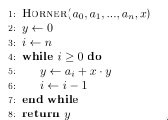
\includegraphics[scale=0.85]{1/Hornet.jpg}
\end{center}
}

\nt{Per individuare l'invariante si prendono in considerazione i valori delle variabili alla riga 3 (inizializzazione) e alla riga 6 (mantenimento).}

\begin{center}
    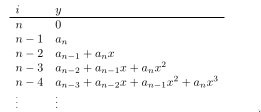
\includegraphics[scale=1]{1/Table.jpg}
\end{center}



\subsubsection{Da ciò si può dedurre che la relazione tra $i$ e $y$, ossia l'\textit{invariante di ciclo} è:}

$$y = \sum_{k = 0}^{n - (i + 1)} a_{k + i + 1} x^k$$

\paragraph{Dimostrazione:} con $y = 0$ e $i = n$ l'invariante è soddisfatto (prima di eseguire il ciclo). Per dimostrare il dopo aggiungiamo $y'$ e $i'$ (i valori aggiornati):

$$i' = i - 1,\:\: i = i' + 1, \:\: y' = a_i + x y$$

\subsubsection{Così si può scrivere:}

$$y' = a_i + x \sum_{k = 0}^{n - (i + 1)} a_{k + i + 1} x^k$$

\subsubsection{Si porta $x$ dentro la sommatoria:}

$$y' = a_i + \sum_{k = 0}^{n - (i + 1)} a_{k + i + 1} x^{k + 1}$$

\subsubsection{Si introducono $k' = k + 1$ e $k = k' - 1$:}

$$y' = a_i + \sum_{k' = 1}^{n - i} a_{k' + i} x^{k'}$$

\subsubsection{Così si può portare dentro alla sommatoria $a_i$:}

$$y' = \sum_{k' = 0}^{n - i} a_{k'+ i} x^{k'}$$

\subsubsection{Infine:}

$$y' = \sum_{k' = 0}^{n - (i' + 1)} a_{k'+ i' + 1} x^{k'}$$

\subsubsection{Il ché è equivalente a:}


$$y = \sum_{k = 0}^{n - (i + 1)} a_{k + i + 1} x^k$$

\subsection{Accenni di terminazione}

Non esiste alcun algoritmo in grado di decidere se data una procedura ed un ingresso la procedura termina (Halting problem). 
In generale è facile avere delle procedure che non terminino, per esempio esistono algoritmi che terminano se l'input rispetta determinate caratteristiche (e. g. è intero), ma non termina se ne ha altre (e.g. è razionale).


